\chapter{Kiến thức cơ sở xác suất và thống kê}\label{ch:1}
\section{Biến ngẫu nhiên và xác suất}\label{sec:1.1}
Biến ngẫu nhiên là một hàm ánh xạ với đặc điểm nó gán một giá trị bằng số cho kết quả đầu ra của một phép thử ngẫu nhiên.
\begin{align}
    \textbf{X}(\alpha)=\textit{x}
\end{align}
với $\alpha$ là đại diện cho đầu ra của một thực nghiệm, \textit{x} là một số thực (hay sự kiện), \textbf{X} là hàm ánh xạ (hay biến ngẫu nhiên).  
Tính ngẫu nhiên được thể hiện ở tham số đầu vào $\alpha$. Điều này dẫn đến đầu ra của hàm là ngẫu nhiên.\\
Đây chưa phải là định nghĩa đầy đủ của một biến ngẫu nhiên. Khái niệm khác liên quan đến định nghĩa của một biến ngẫu nhiên là khái niệm xác suất. \\
Xét một số thí dụ sau.
\begin{itemize}
    \item Gieo một đồng xu trên mặt phẳng, đây là một phép thử. Kết quả có thể xảy ra là "sấp" hoặc "ngửa". Như vậy xác suất cho sự xuất hiện của "sấp" và "ngửa" lần lượt là 
	$ \frac{1}{2} $ và $ \frac{1}{2} $
	\begin{figure}[H]
		\centering
		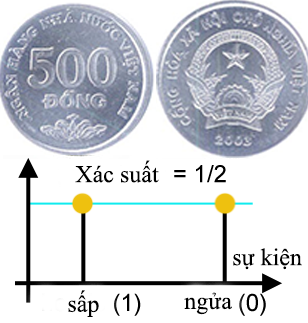
\includegraphics[width=0.4\textwidth]{coin.png}
		\caption{Các sự kiện có thể xuất hiện khi gieo đồng xu}
		\label{fig:web}
	   \end{figure}
    \item Gieo một con súc sắc, đây là một phép thử. Kết quả có thể xảy ra là "Xuất hiện mặt k chấm" tương ứng với k = 1,2,3,..,6. Xác suất cho mỗi sự kiện "Xuất hiện k chấm" đều là $ \frac{1}{6} $.
    \begin{figure}[H]
		\centering
		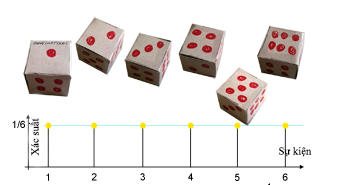
\includegraphics[width=0.6\textwidth]{xucxac.png}
		\caption{Các sự kiện có thể xuất hiện khi gieo súc sắc}
		\label{fig:web}
	   \end{figure}
\end{itemize}
Tổng quát, nếu một phép thử tạo ra n sự kiện khác nhau và khả năng xảy ra như nhau thì xác suất của mỗi sự kiện là $ \frac{1}{n} $
chúng ta có thể nói rằng nếu kết quả của một quá trình nào đó phải là một trong n kết quả khác nhau. 
\par
\section{Phân phối xác suất}\label{sec:1.2}
\par
\subsection{Hàm khối xác suất của biến rời rạc (PMF)}\label{subsec:1.2.1}
\par
\subsection{Hàm mật độ xác suất của biến liên tục (PDF)}\label{subsec:1.2.2}


